% ============================================================
%  PLAN DE MANAGEMENT PROJET (PMP)
%  Time'Eats — Cellule PMO
%  Projet : Refonte Web — Instance du template P2-05
%  Structure : Guide PMP en 11 sections (CESI MAALSI 2026)
% ============================================================
\documentclass[11pt,a4paper,oneside]{report}
\usepackage{../../style/consulting}
\usepackage{pdflscape}
\usetikzlibrary{arrows.meta,positioning}
\hypersetup{pdftitle={Plan de Management Projet — Refonte Web — Time'Eats PMO}}
\pagestyle{fancy}\fancyhf{}
\renewcommand{\headrulewidth}{0pt}
\fancyhead[L]{\begin{tikzpicture}[remember picture,overlay]
  \draw[cnNavy,line width=0.5pt](0,0)--(\textwidth,0);
\end{tikzpicture}\vspace{2pt}\timeeatslogo\hspace{4pt}\small\textcolor{cnSlate}{Time'Eats \textbf{·} Plan de Management Projet (PMP) --- \textit{Refonte Web}}}
\fancyhead[R]{\small\textcolor{cnSlate}{\thepage}}
\fancyfoot[C]{\tiny\textcolor{cnSlate}{Document confidentiel --- Cellule PMO --- CESI MAALSI 2026}}

\newcommand{\ragV}{\cellcolor{cnGreen!20}\textbf{\textcolor{cnGreen}{Vert}}}
\newcommand{\ragA}{\cellcolor{cnOrange!20}\textbf{\textcolor{cnOrange}{Ambre}}}
\newcommand{\ragR}{\cellcolor{cnRed!20}\textbf{\textcolor{cnRed}{Rouge}}}

\begin{document}\small

\begin{center}
{\LARGE\bfseries\color{cnNavy} Plan de Management Projet}\\[4pt]
\textcolor{cnOrange}{\rule{10cm}{1pt}}\\[4pt]
{\large\color{cnSlate} Phase 2 --- Planification \quad|\quad Projet : \textbf{Refonte Web}}\\[2pt]
{\footnotesize\color{cnSlate}\textit{Document maître --- Référentiel PMO Time'Eats}}
\end{center}

\vspace{4pt}
\renewcommand{\arraystretch}{1.4}
\begin{tabularx}{\textwidth}{L{3.5cm} Y L{3.5cm} Y}
\toprule
\rowcolor{cnNavy}\th{Champ} & \th{Valeur} & \th{Champ} & \th{Valeur} \\
\midrule
Nom du projet   & Refonte Web                  & Version PMP    & 1.0 \\
\rowcolor{cnIce}
Chef de projet  & M. X                    & Date           & 22/04/2026 \\
Sponsor         & Mme Y --- DSI Time'Eats  & ESN partenaire & Sopra Steria (forfait 400 j/h) \\
\rowcolor{cnIce}
Budget total    & 300 K€                       & Durée          & 22/04 --- 30/09/2026 (6 mois) \\
Approche        & Hybride (cadre prédictif + Scrum) & Statut    & En cours (avancement 8\,\%) \\
\bottomrule
\end{tabularx}

% =========================================================
% 1. INTRODUCTION ET CADRAGE
% =========================================================
\section*{1 --- Introduction et cadrage}

\subsection*{1.1 Historique et versions}
\renewcommand{\arraystretch}{1.3}
\begin{tabularx}{\textwidth}{L{2cm} L{3cm} Y L{2.5cm}}
\toprule
\rowcolor{cnNavy}\th{Version} & \th{Date} & \th{Modifications} & \th{Auteur} \\
\midrule
v0.1 & 10/04/2026 & Trame initiale --- cadrage par le CP & M. X \\
\rowcolor{cnIce}
v0.5 & 18/04/2026 & Revue interne DSI (budget, jalons, risques) & M. X / Mme Y \\
v0.9 & 20/04/2026 & Intégration retours Marketing et RSSI & M. X \\
\rowcolor{cnIce}
v1.0 & 22/04/2026 & Version de référence validée en COPIL & Mme Y (sponsor) \\
\bottomrule
\end{tabularx}

\subsection*{1.2 Objet du document}
Ce Plan de Management Projet (PMP) décrit \textbf{comment} le projet \emph{Refonte Web} sera exécuté, surveillé, contrôlé et clôturé. Il intègre les plans subsidiaires (périmètre, délais, coûts, qualité, ressources, communication, risques, approvisionnements, parties prenantes, changements) et les \textbf{lignes de base} (scope, échéancier, coûts) qui serviront de référentiel de mesure de performance. Le PMP est destiné à la DG, à la DSI, au chef de projet, à l'équipe projet, à Sopra Steria et au PMO. Il est mis à jour à chaque événement majeur (changement de scope, dépassement de seuil d'alerte, révision de baseline) et au minimum mensuellement.

\subsection*{1.3 Contexte du projet}
Time'Eats vise pour 2026--2027 : 1\,M de nouveaux clients, 10\,000 restaurants partenaires, 25\,\% de part de marché. Le site \texttt{timeats.fr} actuel n'est ni \emph{responsive}, ni conforme RGAA, ni interfaçable avec le futur écosystème (CRM, apps mobiles). La refonte web est la \textbf{pierre angulaire} de la transformation digitale 2026 : socle commun de l'écosystème via une API publique, levier marketing et commerce, et industrialisation de la production éditoriale par un CMS contributeur. Le projet est inscrit au portefeuille DSI avec un score de priorisation de \textbf{3{,}80 / 5{,}00} (RAG \ragV).

\subsection*{1.4 Analyse SWOT}
\renewcommand{\arraystretch}{1.5}
\begin{tabularx}{\textwidth}{Y Y}
\toprule
\cellcolor{cnGreen!30}\th{Forces (S)} & \cellcolor{cnGreen!30}\th{Faiblesses (W)} \\
\midrule
\cellcolor{cnGreen!10}\textbullet\ Sponsoring fort DSI + DG sur la transformation digitale \newline
\textbullet\ Équipe Tech Lead expérimentée (Next.js, design system) \newline
\textbullet\ Budget sécurisé (300 K€ verrouillés en COPIL) \newline
\textbullet\ Forfait ESN Sopra Steria (transfert risque dépassement) \newline
\textbullet\ Référent Marketing engagé (15\,\% contractualisés)
&
\cellcolor{cnGreen!10}\textbullet\ Dépendance projet Office 365 (SSO espace client) \newline
\textbullet\ Équipe DSI déjà très sollicitée par 11 projets simultanés \newline
\textbullet\ Pas de design system existant (à créer) \newline
\textbullet\ Compétences accessibilité (RGAA) externes uniquement \newline
\textbullet\ Historique de retards sur les projets web précédents \\
\midrule
\cellcolor{cnOrange!30}\th{Opportunités (O)} & \cellcolor{cnOrange!30}\th{Menaces (T)} \\
\midrule
\cellcolor{cnOrange!10}\textbullet\ API publique réutilisable par CRM et apps mobiles (mutualisation) \newline
\textbullet\ Vitrine projet PMO (référence pour les autres projets) \newline
\textbullet\ Préparer campagne marketing nationale Q4 2026 \newline
\textbullet\ Réduction TCO de 25\,\% sur 12 mois \newline
\textbullet\ Audit RGAA valorisable (image responsable + marchés publics)
&
\cellcolor{cnOrange!10}\textbullet\ Glissement du projet Office 365 (impact SSO) \newline
\textbullet\ Dérive de scope sur CMS (contenu legacy) \newline
\textbullet\ Cyberattaque (site vitrine = surface d'attaque) \newline
\textbullet\ Non-conformité RGAA $\Rightarrow$ sanction CNIL + image \newline
\textbullet\ Concurrents en avance sur la transition digitale \\
\bottomrule
\end{tabularx}

\subsection*{1.5 Enjeux et objectifs SMART --- Arbre des objectifs}
Chaque objectif est formulé selon la méthode \textbf{SMART} (Spécifique, Mesurable, Atteignable, Réaliste, Temporel).

\renewcommand{\arraystretch}{1.4}
\begin{tabularx}{\textwidth}{C{0.7cm} L{2.6cm} Y C{2.4cm} C{2cm}}
\toprule
\rowcolor{cnNavy}\th{N°} & \th{Enjeu} & \th{Objectif SMART} & \th{Indicateur} & \th{Échéance} \\
\midrule
O1 & Croissance commerciale & Atteindre +30\,\% de trafic organique vs T1 2026 & Sessions / mois Analytics & M+6 post Go-Live \\
\rowcolor{cnIce}
O2 & Expérience client & Lighthouse Performance et A11y $\geq$ 90 sur 10 parcours-clés & Score Lighthouse & Go-Live (30/09/2026) \\
O3 & Industrialisation & Réduire de 5j à $<$ 30 min le délai de mise en ligne d'un contenu & Temps moyen CMS & M+3 post Go-Live \\
\rowcolor{cnIce}
O4 & Écosystème digital & Livrer API publique REST v1 documentée (OpenAPI 3) & API en production & 30/06/2026 (J2) \\
O5 & Conformité \& éthique & Atteindre RGAA 4.1 niveau AA et OWASP ASVS niveau 2 & Rapports d'audit & 31/08/2026 (J4) \\
\rowcolor{cnIce}
O6 & TCO & Baisser le coût total de possession de 25\,\% à 12 mois & Comptabilité analytique & M+12 \\
\bottomrule
\end{tabularx}

\vspace{6pt}
\begin{reco}
L'arbre des objectifs ci-dessous (généré par PlantUML) décompose l'objectif global \og soutenir la croissance nationale\fg{} en cinq familles d'objectifs opérationnels mesurables. Il sert de support de négociation avec le sponsor et de fil rouge en COPIL.
\end{reco}

\begin{center}
  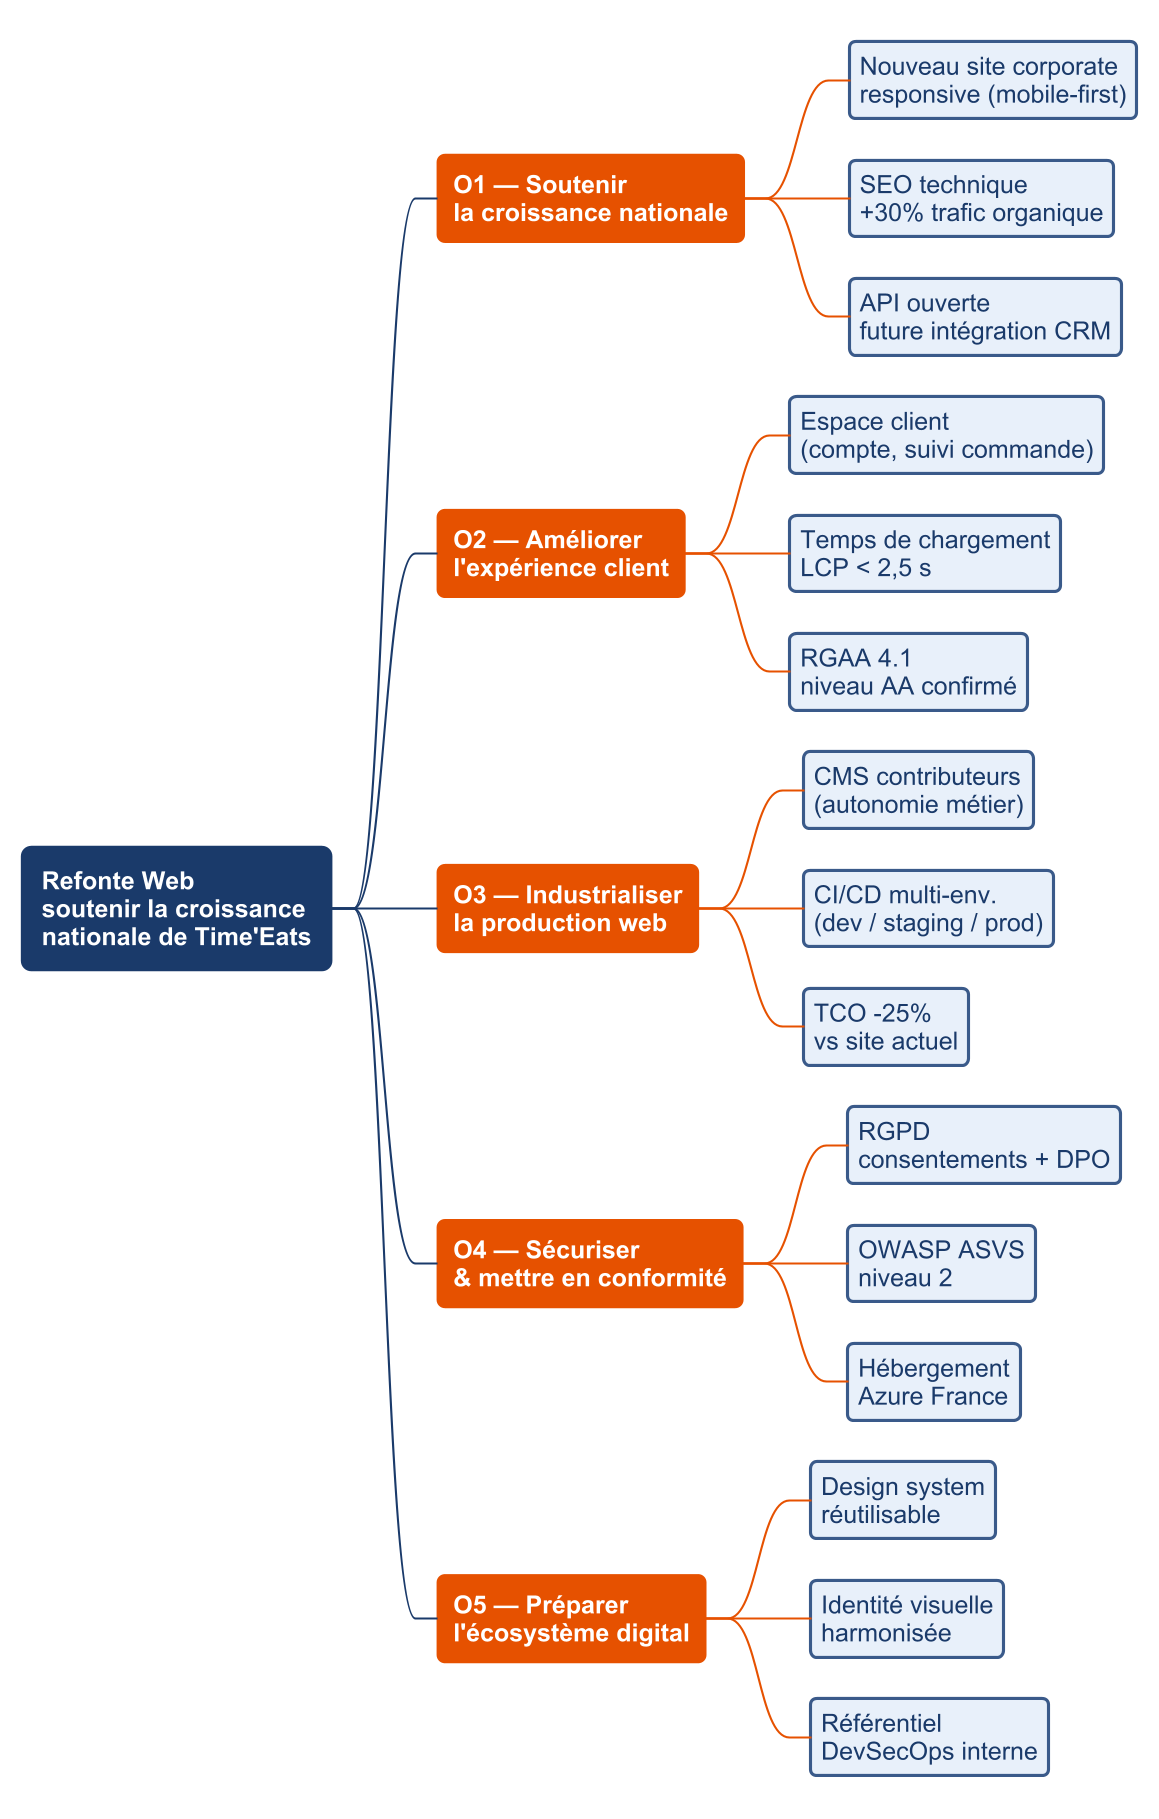
\includegraphics[width=0.95\textwidth,keepaspectratio]{../../diagrammes/arbre_objectifs_refonte_web.png}
  \par\vspace{4pt}
  {\footnotesize\textcolor{cnSlate}{\textit{Arbre des objectifs --- Refonte Web (source : \texttt{arbre\_objectifs\_refonte\_web.puml})}}}
\end{center}

\subsection*{1.6 Triangle d'Or --- arbitrage Coût / Délai / Qualité}

Le \textbf{Triangle d'Or} formalise les contraintes croisées du projet et sert d'outil de négociation : toute modification d'un axe impacte les deux autres.

\vspace{6pt}
\begin{center}
\begin{tikzpicture}[scale=1.1]
  \coordinate (C) at (0,3.4);     % Coût (haut)
  \coordinate (D) at (-3,-1.8);   % Délai (bas gauche)
  \coordinate (Q) at (3,-1.8);    % Qualité (bas droit)
  \draw[cnNavy, line width=1.8pt, fill=cnIce] (C) -- (D) -- (Q) -- cycle;
  \node[fill=cnNavy, text=white, rounded corners=4pt, inner sep=6pt, font=\bfseries] at (C) {Coût --- 300 K€};
  \node[fill=cnNavy, text=white, rounded corners=4pt, inner sep=6pt, font=\bfseries] at (D) {Délai --- 30/09/2026};
  \node[fill=cnNavy, text=white, rounded corners=4pt, inner sep=6pt, font=\bfseries] at (Q) {Qualité / Périmètre};
  \node[align=center, font=\small\itshape, text=cnSlate] at (0,0.4) {Priorité projet :\\\textbf{Délai > Qualité > Coût}};
  \node[text=cnOrange, font=\small\bfseries] at (-2.4,0.9) {Forfait ESN};
  \node[text=cnOrange, font=\small\bfseries] at (2.4,0.9) {RGAA AA};
  \node[text=cnOrange, font=\small\bfseries] at (0,-2.3) {Go-Live impératif Q4};
\end{tikzpicture}
\end{center}

\vspace{4pt}
\textbf{Règles d'arbitrage :}

\renewcommand{\arraystretch}{1.4}
\begin{tabularx}{\textwidth}{L{4cm} Y}
\toprule
\rowcolor{cnNavy}\th{Si pression sur...} & \th{Alors arbitrage retenu} \\
\midrule
Délai (Go-Live) & \textbf{Priorité absolue} : aucun glissement de J5 toléré. Si dépassement risqué, réduire le périmètre fonctionnel (espace client minimal, CMS Phase 2) plutôt que repousser. \\
\rowcolor{cnIce}
Coût (300 K€) & Enveloppe ferme. Tout dépassement requiert avenant COPIL + financement complémentaire DG. \\
Qualité / Périmètre & Le socle RGAA AA, OWASP ASVS 2 et API v1 documentée est \textbf{non négociable}. Les fonctionnalités secondaires (newsletter, blog, témoignages) peuvent glisser en Phase 2 si pression budget ou délai. \\
\bottomrule
\end{tabularx}

% =========================================================
% 2. PÉRIMÈTRE
% =========================================================
\newpage
\section*{2 --- Périmètre du projet (Scope)}

\subsection*{2.1 Périmètre fonctionnel, technique et géographique}
\renewcommand{\arraystretch}{1.3}
\begin{tabularx}{\textwidth}{L{3cm} Y}
\toprule
\rowcolor{cnNavy}\th{Dimension} & \th{Couverture} \\
\midrule
Fonctionnel    & Site corporate vitrine + CMS contributeur + espace client (compte, suivi commande, factures, préférences) + API publique REST v1 (catalogue, recherche, contact, comptes). \\
\rowcolor{cnIce}
Technique      & Front : Next.js 14, TypeScript ; Back : Node.js (NestJS) + PostgreSQL ; Headless CMS (Strapi ou Directus, à arbitrer en J2) ; Auth : SSO Office 365 (repli IdP local Keycloak) ; Hébergement : Azure West Europe (Paris) ; CI/CD : GitHub Actions + Azure Pipelines ; APM : Application Insights. \\
Géographique   & Marché français en V1 ; \emph{i18n}-ready (architecture multilingue prête, langues additionnelles hors scope V1). \\
\rowcolor{cnIce}
Utilisateurs   & Visiteurs prospects, clients particuliers (B2C), contributeurs Marketing/Communication (CMS), équipes Commerce (lecture API), Service Client (consultation comptes). \\
\bottomrule
\end{tabularx}

\subsection*{2.2 Domaines inclus (IN)}
\begin{itemize}
  \item Audit UX/SEO du site actuel + benchmarks concurrence.
  \item Création du \textbf{design system} (composants, tokens, librairie Storybook).
  \item Refonte de \textbf{10 templates de page} (accueil, catégorie, produit, recherche, contact, blog, CGU, mentions légales, profil, suivi commande).
  \item CMS contributeur : gestion contenus, médias, SEO meta, multi-utilisateurs avec rôles.
  \item Espace client : création compte, login (SSO ou local), profil, historique commandes (lecture API CRM-prêt), factures, préférences.
  \item API publique REST v1 : 12 endpoints documentés OpenAPI 3 (catalogue, recherche, contact, comptes, sessions, articles).
  \item SEO technique : balisage Schema.org, sitemap, robots, Core Web Vitals, redirections legacy.
  \item Conformité \textbf{RGAA 4.1 niveau AA} : audit avant Go-Live, mise en accessibilité.
  \item Conformité \textbf{RGPD} : registre traitements, consentements, droits d'accès / suppression.
  \item Sécurité \textbf{OWASP ASVS niveau 2} : audit avant Go-Live, durcissement.
  \item \textbf{CI/CD} multi-environnement (dev / staging / prod) avec promotion automatique sur tag.
  \item \textbf{Monitoring} : Application Insights, alerting sur SLO (uptime $\geq$ 99{,}5\,\%, error rate $<$ 1\,\%).
  \item Documentation utilisateur (contributeurs CMS) et technique (équipe Run).
\end{itemize}

\subsection*{2.3 Domaines exclus (OUT)}
\begin{itemize}
  \item Refonte CRM (projet dédié, démarrage juin 2026).
  \item Applications mobiles Clients et Fournisseurs (projets séparés).
  \item Tunnel de commande B2B avancé (Phase 2 post-Go-Live).
  \item Back-office logistique et gestion des stocks (couvert par le futur CRM).
  \item Refonte de l'intranet collaborateur Time'Eats.
  \item Migration des contenus legacy antérieurs à 2024 (à statuer en avenant si demandé).
  \item Versions multilingues (anglais, espagnol) : architecture \emph{i18n}-ready prête, traduction hors scope.
\end{itemize}

% =========================================================
% 3. GOUVERNANCE ET ORGANISATION
% =========================================================
\newpage
\section*{3 --- Gouvernance et organisation}

\subsection*{3.1 Sponsor}
\textbf{Sponsor exécutif :} Mme Y, Directrice des Systèmes d'Information (DSI). Garant politique, financier et arbitre des escalades. Présidente du COPIL mensuel. \\
\textbf{Autorité ultime :} M. Z, Directeur Général --- arbitrage en cas de dépassement de budget ou de glissement de jalon majeur.

\subsection*{3.2 Équipe projet}
\renewcommand{\arraystretch}{1.3}
\begin{tabularx}{\textwidth}{L{4cm} L{3cm} Y C{2cm}}
\toprule
\rowcolor{cnNavy}\th{Membre} & \th{Rôle} & \th{Mission} & \th{Aff.} \\
\midrule
M. X     & Chef de projet     & Pilotage global, COPIL, gestion ESN & 50\,\% \\
\rowcolor{cnIce}
M. A    & Tech Lead Front    & Architecture front, design system, code review & 60\,\% \\
M. B      & Dev Back-End       & API, intégrations CRM-ready, sécurité applicative & 60\,\% \\
\rowcolor{cnIce}
Mme C   & UX/UI Designer     & Wireframes, maquettes Figma, design system & 80\,/30\,\% \\
M. D     & DevOps             & Pipeline CI/CD, environnements, monitoring & 20\,\% \\
\rowcolor{cnIce}
Mme E    & RSSI               & Validation sécurité, audit OWASP & 10\,\% \\
Mme F      & Resp. Marketing    & Référent métier MOA, validation contenus & 15\,\% \\
\rowcolor{cnIce}
M. G    & Lead tech ESN      & Architecture cible, sécurisation forfait & 80 j/h \\
Sopra Steria  & ESN forfait        & 2 devs front + 2 devs back + UX expert + QA & 320 j/h \\
\bottomrule
\end{tabularx}

\subsection*{3.3 Organigramme projet}
\begin{center}
  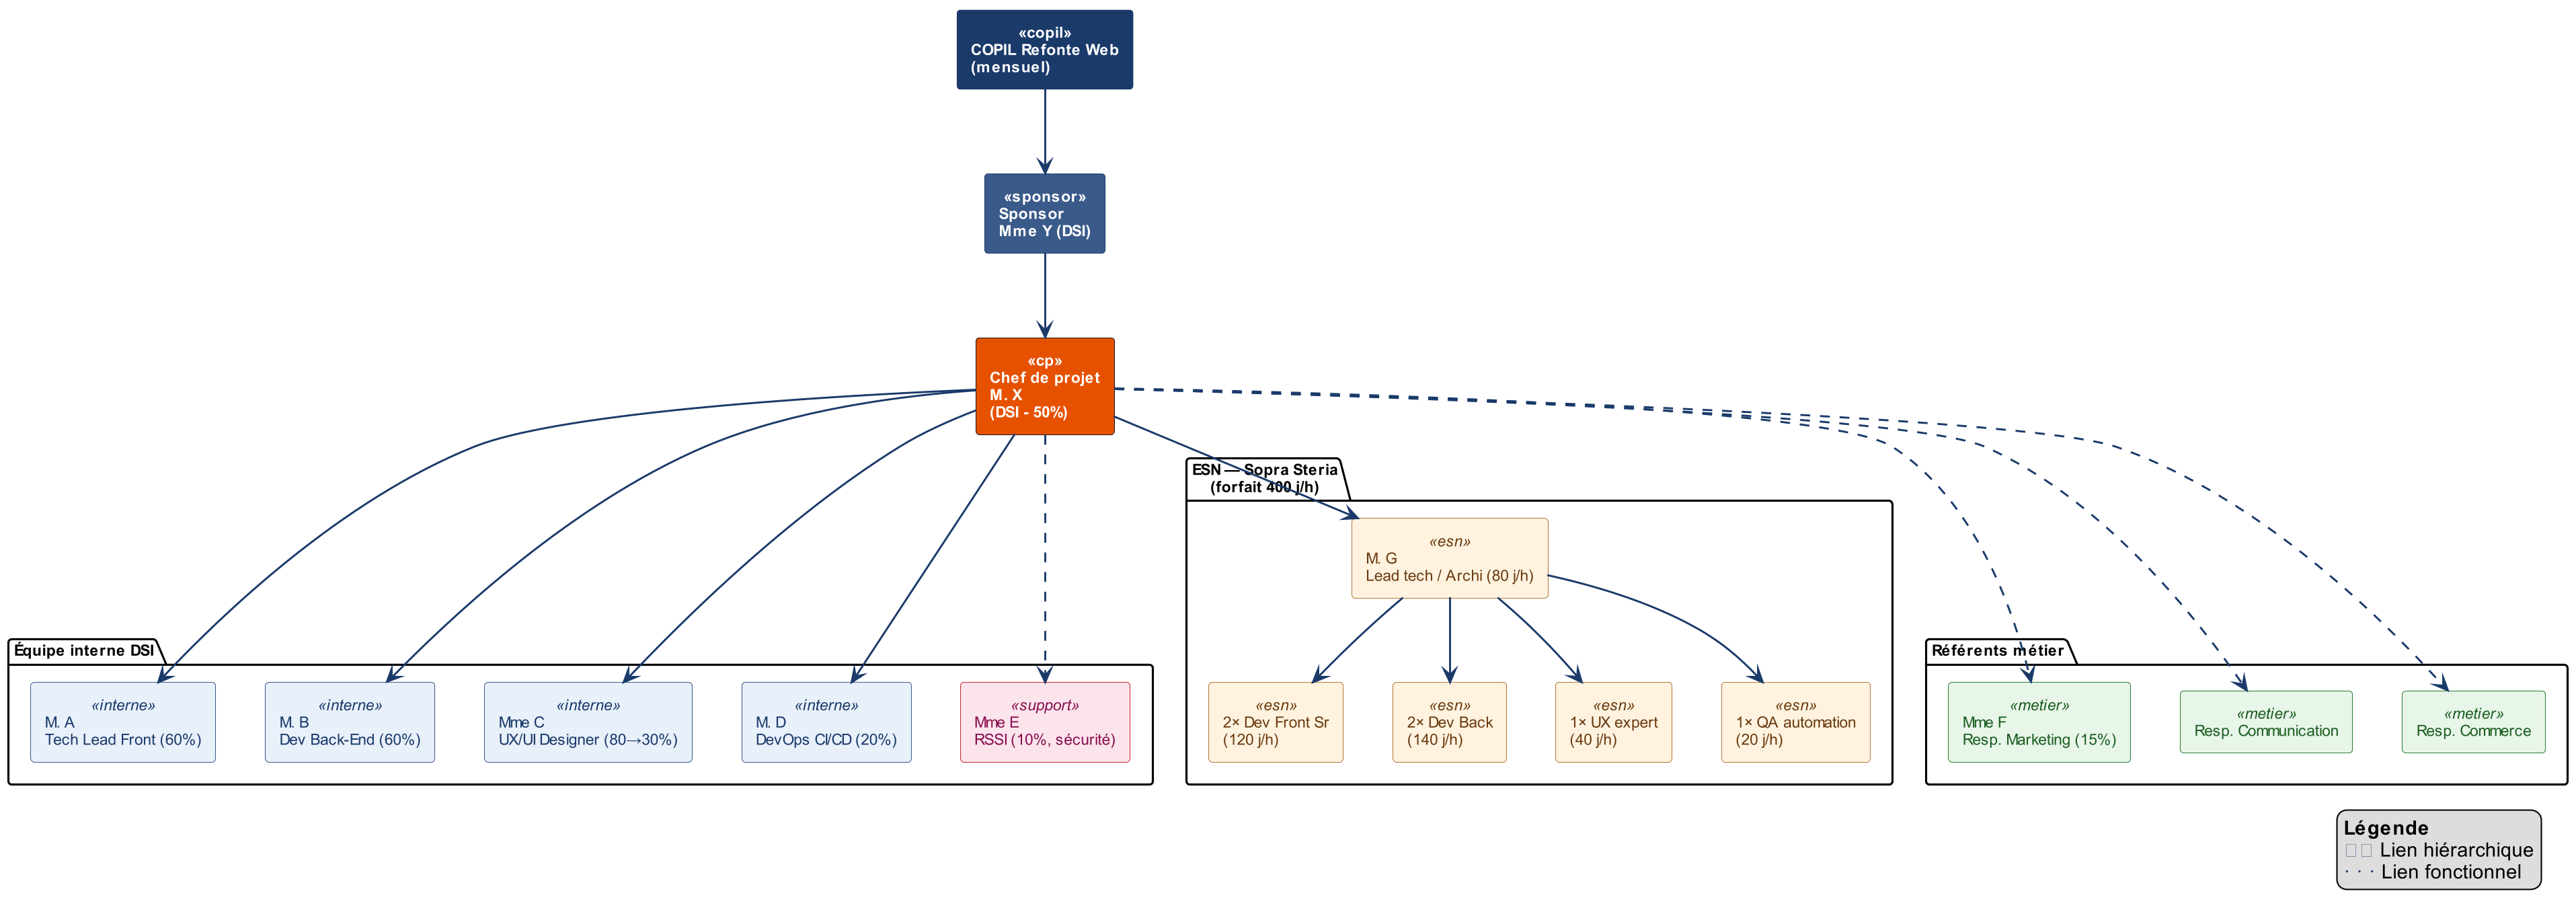
\includegraphics[width=0.92\textwidth,keepaspectratio]{../../diagrammes/organigramme_refonte_web.png}
  \par\vspace{4pt}
  {\footnotesize\textcolor{cnSlate}{\textit{Organigramme projet Refonte Web (source : \texttt{organigramme\_refonte\_web.puml})}}}
\end{center}

\subsection*{3.4 Matrice RACI}
La matrice RACI complète couvrant les 5 phases du projet est rédigée dans le document compagnon \textbf{P1-04 --- Matrice RACI}. Règle PMO : un seul \textbf{A} par activité, au moins un \textbf{R} par activité.

\subsection*{3.5 Instances de pilotage}
\renewcommand{\arraystretch}{1.4}
\begin{tabularx}{\textwidth}{L{3.5cm} L{2.5cm} Y}
\toprule
\rowcolor{cnNavy}\th{Instance} & \th{Fréquence} & \th{Participants \& objectifs} \\
\midrule
COPIL Refonte Web      & Mensuel (3\textsuperscript{e} mardi 9h) & Sponsor DSI + CP + Tech Lead + Lead ESN + Resp. Marketing. Validation jalons, arbitrage écarts ($>$ 5\,\% budget ou $>$ 10 j délai). \\
\rowcolor{cnIce}
Revue de sprint (démo) & Toutes les 2 semaines (vendredi 14h) & Équipe projet complète + référents métier. Démo incrément + rétrospective Scrum. \\
Daily Scrum            & Quotidien (9h15 --- 15 min) & Équipe technique (interne + ESN sur sprint). Lever les blocages. \\
\rowcolor{cnIce}
Point hebdo CP / ESN   & Hebdomadaire (mercredi 17h) & M. X + M. G. Suivi forfait, livrables, alertes. \\
Comité Stratégique DSI & Mensuel & Reporting du portefeuille (le projet y est consolidé via le Cockpit DSI). \\
\bottomrule
\end{tabularx}

\subsection*{3.6 Cartographie des parties prenantes (Pouvoir × Intérêt)}

\vspace{6pt}
\begin{center}
\begin{tikzpicture}[scale=1.0]
  % Cadrage
  \draw[cnNavy, line width=1.2pt] (0,0) rectangle (10,8);
  \draw[cnSlate, dashed, line width=0.6pt] (5,0) -- (5,8);
  \draw[cnSlate, dashed, line width=0.6pt] (0,4) -- (10,4);
  % Axes
  \node[font=\small\bfseries\color{cnNavy}, anchor=south] at (5,8.2) {Cartographie Pouvoir $\times$ Intérêt};
  \node[font=\small\color{cnSlate}, rotate=90, anchor=south] at (-0.4,4) {Pouvoir $\longrightarrow$};
  \node[font=\small\color{cnSlate}, anchor=north] at (5,-0.2) {Intérêt $\longrightarrow$};
  % Quadrants labels
  \node[font=\footnotesize\itshape\color{cnSlate}, align=center] at (2.5,7.6) {Tenir informés};
  \node[font=\footnotesize\itshape\color{cnSlate}, align=center] at (7.5,7.6) {Gérer de près};
  \node[font=\footnotesize\itshape\color{cnSlate}, align=center] at (2.5,0.4) {Surveiller};
  \node[font=\footnotesize\itshape\color{cnSlate}, align=center] at (7.5,0.4) {Maintenir satisfaits};
  % Stakeholders dots
  \node[fill=cnOrange, text=white, circle, inner sep=2pt, font=\tiny\bfseries] at (8.5,7) {DG};
  \node[fill=cnOrange, text=white, circle, inner sep=2pt, font=\tiny\bfseries] at (8.8,6) {DSI};
  \node[fill=cnNavy, text=white, circle, inner sep=2pt, font=\tiny\bfseries] at (7.8,5.5) {CP};
  \node[fill=cnOrange, text=white, circle, inner sep=2pt, font=\tiny\bfseries] at (7.2,4.7) {ESN};
  \node[fill=cnGreen, text=white, circle, inner sep=2pt, font=\tiny\bfseries] at (8.0,3.6) {Marketing};
  \node[fill=cnGreen, text=white, circle, inner sep=2pt, font=\tiny\bfseries] at (6.5,3.2) {Commerce};
  \node[fill=cnNavy, text=white, circle, inner sep=2pt, font=\tiny\bfseries] at (3.0,5.8) {RSSI};
  \node[fill=cnNavy, text=white, circle, inner sep=2pt, font=\tiny\bfseries] at (3.2,4.6) {DPO};
  \node[fill=cnGreen, text=white, circle, inner sep=2pt, font=\tiny\bfseries] at (7.4,2.4) {Service Client};
  \node[fill=cnSlate, text=white, circle, inner sep=2pt, font=\tiny\bfseries] at (2.0,1.6) {Visiteurs};
  \node[fill=cnSlate, text=white, circle, inner sep=2pt, font=\tiny\bfseries] at (3.2,2.6) {Clients B2C};
  \node[fill=cnSlate, text=white, circle, inner sep=2pt, font=\tiny\bfseries] at (1.5,3.0) {Hébergeur Azure};
\end{tikzpicture}
\end{center}

\textbf{Stratégies de communication associées :} \emph{Gérer de près} = COPIL, briefings ; \emph{Tenir informés} = newsletters internes ; \emph{Maintenir satisfaits} = revues de sprint, démos ; \emph{Surveiller} = communication broadcast, FAQ.

% =========================================================
% 4. PLANIFICATION ET LIVRABLES
% =========================================================
\newpage
\section*{4 --- Planification et livrables}

\subsection*{4.1 PBS --- Product Breakdown Structure}

Le PBS décompose le \textbf{produit livré} (par opposition au WBS qui décompose le \textbf{travail}). Il sert de référence pour la recette et le transfert run.

\renewcommand{\arraystretch}{1.3}
\begin{tabularx}{\textwidth}{C{1.5cm} L{4cm} Y}
\toprule
\rowcolor{cnNavy}\th{Code PBS} & \th{Composant produit} & \th{Description} \\
\midrule
PBS-1 & Site corporate                & 10 templates de page, navigation, recherche, SEO \\
\rowcolor{cnIce}
PBS-2 & Espace client                 & Compte, login, profil, historique, factures \\
PBS-3 & CMS contributeur              & Backoffice headless, gestion contenus + médias + SEO meta \\
\rowcolor{cnIce}
PBS-4 & API publique REST v1          & 12 endpoints OpenAPI 3, SDK JS optionnel \\
PBS-5 & Design system                 & Librairie Storybook (composants + tokens + guidelines) \\
\rowcolor{cnIce}
PBS-6 & Pipeline CI/CD                & Environnements dev/staging/prod + promotion + tests \\
PBS-7 & Documentation                 & Manuel contributeur CMS + doc technique Run + ADR \\
\rowcolor{cnIce}
PBS-8 & Audit \& conformité           & Rapports RGAA AA, OWASP ASVS 2, performance Lighthouse \\
\bottomrule
\end{tabularx}

\subsection*{4.2 WBS --- Work Breakdown Structure}
Le WBS détaillé (tabulaire + graphique) est dans le document compagnon \textbf{P2-06 --- WBS}. Il décompose le projet en \textbf{8 lots} et \textbf{34 work packages}. La représentation graphique est produite par PlantUML.

\subsection*{4.3 Macro-planning et planning détaillé}
Le diagramme de Gantt baseline (vues macro et détaillée par sprint Scrum) est dans le document compagnon \textbf{P2-07 --- Planning Gantt}. Cadence sprint : 2 semaines. Total : 11 sprints S1--S11.

\subsection*{4.4 Jalons majeurs}
\renewcommand{\arraystretch}{1.4}
\begin{tabularx}{\textwidth}{C{1cm} L{5cm} Y C{2cm}}
\toprule
\rowcolor{cnNavy}\th{N°} & \th{Jalon} & \th{Critère de passage} & \th{Date} \\
\midrule
J0 & Démarrage officiel       & Charte signée + équipe staffée + kick-off réalisé & 22/04/2026 \\
\rowcolor{cnIce}
J1 & Maquettes UX validées    & Design system v1 + 5 parcours-clés signés métier & 27/05/2026 \\
J2 & Socle technique validé   & Architecture validée + API v1 documentée + CI/CD opérationnel & 30/06/2026 \\
\rowcolor{cnIce}
J3 & MVP fonctionnel          & Site + CMS + espace client min. en staging --- démo MOA OK & 31/07/2026 \\
J4 & Recette + RGAA           & PV de recette signé + audit RGAA AA réussi & 31/08/2026 \\
\rowcolor{cnIce}
J5 & Go-Live + Clôture        & Bascule production + transfert run + REX rédigé & 30/09/2026 \\
\bottomrule
\end{tabularx}

\subsection*{4.5 Liste des livrables et critères d'acceptation}
\renewcommand{\arraystretch}{1.3}
\begin{tabularx}{\textwidth}{L{3.5cm} Y C{2cm}}
\toprule
\rowcolor{cnNavy}\th{Livrable} & \th{Critère d'acceptation} & \th{Échéance} \\
\midrule
Charte projet (P1-01)         & Signée par CP / DSI / DG & J0 \\
\rowcolor{cnIce}
PMP (ce document)             & Validé en COPIL d'avril & 22/04 \\
Wireframes + design system v1 & 5 parcours principaux + 30 composants Storybook & J1 \\
\rowcolor{cnIce}
API REST v1                   & 12 endpoints, doc OpenAPI 3, tests $>$ 80\,\% & J2 \\
Pipeline CI/CD                & Déploiement auto staging on push, prod on tag & J2 \\
\rowcolor{cnIce}
Site corporate                & 10 templates de page, contenu validé Marketing & J3 \\
CMS contributeur              & 3 rôles, multi-utilisateurs, doc utilisateur livrée & J3 \\
\rowcolor{cnIce}
Espace client                 & Login SSO/local + profil + historique commandes & J3 \\
Audit RGAA 4.1                & Score $\geq$ niveau AA, rapport éditeur certifié & J4 \\
\rowcolor{cnIce}
Audit OWASP ASVS 2            & Aucune vulnérabilité critique ouverte & J4 \\
Tests performance             & Lighthouse Perf $\geq$ 90, A11y $\geq$ 90 sur 10 parcours & J4 \\
\rowcolor{cnIce}
Bascule production (Go-Live)  & SLO uptime $\geq$ 99{,}5\,\%, monitoring en place & J5 \\
PV de transfert run           & Signé DSI Ops + équipe Run formée & J5 \\
\rowcolor{cnIce}
Fiche REX                     & Sessions REX tenues, capitalisations classées PMO & J5 \\
\bottomrule
\end{tabularx}

% =========================================================
% 5. RESSOURCES ET BUDGET
% =========================================================
\newpage
\section*{5 --- Gestion des ressources et budget}

\subsection*{5.1 Dimensionnement RH}
Effectif total cumulé : \textbf{4{,}5 ETP internes} + \textbf{400 j/h ESN Sopra Steria} sur 6 mois (équivalent $\approx$ 4 ETP ESN). Tableau RH détaillé : voir §3.2.

\subsection*{5.2 Ressources matérielles}
\begin{itemize}
  \item \textbf{Environnements cloud} : Azure West Europe --- 3 environnements (dev, staging, prod) --- estimé 1\,K€/mois.
  \item \textbf{Licences logicielles} : CMS headless (Strapi Cloud ou Directus Pro) --- 6 K€/an ; Figma équipe (10 sièges) --- 1{,}5 K€/an ; outils de monitoring (Application Insights, Sentry) --- inclus Azure.
  \item \textbf{Outillage} : repo GitHub Enterprise (existant), Jira (existant), Confluence (existant).
  \item \textbf{Postes de travail} : équipe interne équipée ; ESN apporte son matériel.
\end{itemize}

\subsection*{5.3 Budget prévisionnel synthétique}
Le détail par poste mensuel est dans le document compagnon \textbf{P2-08 --- Budget prévisionnel}. Synthèse :

\renewcommand{\arraystretch}{1.3}
\begin{tabularx}{\textwidth}{L{6cm} C{2.5cm} C{2cm} Y}
\toprule
\rowcolor{cnNavy}\th{Poste} & \th{Montant} & \th{\% total} & \th{Nature} \\
\midrule
ESN Sopra Steria (forfait 400 j/h)    & 200 K€ & 67\,\% & Externe \\
\rowcolor{cnIce}
Interne DSI (valorisation j/h)        &  80 K€ & 27\,\% & Interne \\
Licences (CMS, Figma, monitoring)     &   7 K€ &  2\,\% & Externe \\
\rowcolor{cnIce}
Infrastructure Azure                  &   6 K€ &  2\,\% & Externe \\
Audits externes (RGAA, OWASP)         &   4 K€ &  1\,\% & Externe \\
\rowcolor{cnIce}
Réserve aléas (intégrée par poste)    &   3 K€ &  1\,\% & Réserve \\
\midrule
\rowcolor{cnNavy!15}
\textbf{TOTAL}                        & \textbf{300 K€} & \textbf{100\,\%} & \\
\bottomrule
\end{tabularx}

% =========================================================
% 6. COMMUNICATION
% =========================================================
\newpage
\section*{6 --- Plan de communication}

\subsection*{6.1 Contenus et cibles}
\renewcommand{\arraystretch}{1.4}
\begin{tabularx}{\textwidth}{L{3cm} L{3.5cm} Y}
\toprule
\rowcolor{cnNavy}\th{Cible} & \th{Contenu} & \th{Objectif} \\
\midrule
DG / sponsor       & Synthèse RAG + écarts + arbitrages & Décider, sponsoriser \\
\rowcolor{cnIce}
COPIL              & Tableau de bord + jalons + risques & Arbitrer \\
Équipe projet      & Sprint backlog, démos, rétro & Aligner, livrer \\
\rowcolor{cnIce}
ESN Sopra Steria   & Backlog forfait, livrables, paiements & Piloter \\
Métiers (Marketing, Commerce) & Démos, contenus à valider & Co-construire \\
\rowcolor{cnIce}
DSI Ops / Run      & Documentation transfert, formation & Prendre la main au Go-Live \\
Collaborateurs internes & Annonces Go-Live, formation CMS & Adopter, contribuer \\
\rowcolor{cnIce}
Clients / prospects & Annonce Go-Live (newsletter, presse) & Engager, convertir \\
\bottomrule
\end{tabularx}

\subsection*{6.2 Moyens et outils}
\begin{itemize}
  \item \textbf{Teams} : canaux dédiés (équipe, ESN, métiers).
  \item \textbf{SharePoint Online} : référentiel documentaire PMO + dossier projet.
  \item \textbf{Jira} : backlog Scrum, suivi anomalies.
  \item \textbf{Confluence} : documentation technique, ADR.
  \item \textbf{Cockpit DSI} : tableau de bord temps réel, RAG, KPIs.
  \item \textbf{COPIL} en présentiel + Teams pour les distants.
  \item \textbf{Newsletter interne} : Time'Eats Hebdo (relais des annonces Go-Live).
\end{itemize}

\subsection*{6.3 Fréquence et formats}
Voir document compagnon \textbf{P2-10 --- Plan de communication} pour le détail fréquence × canal × destinataire.

% =========================================================
% 7. RISQUES
% =========================================================
\newpage
\section*{7 --- Gestion des risques}

\subsection*{7.1 Cartographie des risques (probabilité × impact)}

\vspace{6pt}
\begin{center}
\begin{tikzpicture}[scale=1.05]
  % Heatmap 5x5
  \foreach \x in {1,...,5} {
    \foreach \y in {1,...,5} {
      \pgfmathsetmacro{\score}{\x*\y}
      \pgfmathsetmacro{\color}{ifthenelse(\score<6,"cnGreen!30",ifthenelse(\score<13,"cnOrange!30","cnRed!30"))}
      \draw[fill=\color, draw=cnSlate, line width=0.4pt] (\x-1,\y-1) rectangle (\x,\y);
    }
  }
  % Axes
  \foreach \i in {1,...,5} {
    \node[font=\footnotesize\color{cnNavy}] at (\i-0.5,-0.4) {\i};
    \node[font=\footnotesize\color{cnNavy}] at (-0.4,\i-0.5) {\i};
  }
  \node[font=\small\bfseries\color{cnNavy}, anchor=north] at (2.5,-0.9) {Probabilité $\longrightarrow$};
  \node[font=\small\bfseries\color{cnNavy}, rotate=90, anchor=south] at (-0.9,2.5) {Impact $\longrightarrow$};
  % Risk points
  \node[fill=cnNavy, text=white, circle, inner sep=2pt, font=\tiny\bfseries] at (3.0,4.0) {R1};
  \node[fill=cnNavy, text=white, circle, inner sep=2pt, font=\tiny\bfseries] at (2.0,5.0) {R2};
  \node[fill=cnNavy, text=white, circle, inner sep=2pt, font=\tiny\bfseries] at (3.0,4.0) {};
  \node[fill=cnNavy, text=white, circle, inner sep=2pt, font=\tiny\bfseries] at (3.4,3.6) {R3};
  \node[fill=cnNavy, text=white, circle, inner sep=2pt, font=\tiny\bfseries] at (4.0,3.0) {R4};
  \node[fill=cnNavy, text=white, circle, inner sep=2pt, font=\tiny\bfseries] at (3.0,3.0) {R5};
  \node[fill=cnNavy, text=white, circle, inner sep=2pt, font=\tiny\bfseries] at (1.0,5.0) {R6};
  \node[fill=cnNavy, text=white, circle, inner sep=2pt, font=\tiny\bfseries] at (2.0,4.0) {R7};
  % Legend
  \node[fill=cnGreen!30, draw=cnSlate, rounded corners=2pt, font=\tiny] at (6.5,4.4) {Faible};
  \node[fill=cnOrange!30, draw=cnSlate, rounded corners=2pt, font=\tiny] at (6.5,3.8) {Moyen};
  \node[fill=cnRed!30, draw=cnSlate, rounded corners=2pt, font=\tiny] at (6.5,3.2) {Critique};
\end{tikzpicture}
\end{center}

\subsection*{7.2 Registre des risques (top 7)}
\renewcommand{\arraystretch}{1.3}
\begin{tabularx}{\textwidth}{C{0.6cm} L{4.3cm} C{0.7cm} C{0.7cm} C{1.5cm} Y}
\toprule
\rowcolor{cnNavy}\th{ID} & \th{Risque} & \th{P} & \th{I} & \th{Score} & \th{Mitigation} \\
\midrule
R1 & Retard projet Office 365 (SSO espace client)  & 3 & 4 & 12 \ragA & Plan B : IdP local Keycloak (surcoût 8 K€). Décision GO/NO-GO IdP à J2. \\
\rowcolor{cnIce}
R2 & Non-conformité RGAA 4.1 niveau AA              & 2 & 5 & 10 \ragA & Audit blanc S20 + plan d'action. Audit final S23 par cabinet certifié. \\
R3 & Sous-effectif ESN sur sprint critique S22-24   & 3 & 4 & 12 \ragA & Clause contractuelle de continuité d'équipe + pénalités. \\
\rowcolor{cnIce}
R4 & Dérive de scope sur CMS (contenu legacy)        & 4 & 3 & 12 \ragA & Gouvernance changement stricte (§9) + COPIL d'arbitrage. \\
R5 & Indisponibilité référent Marketing (validation) & 3 & 3 &  9 \ragA & 15\,\% temps contractualisé + créneaux fixes (mardis 14-17h). \\
\rowcolor{cnIce}
R6 & Cyberattaque (XSS, injection, DDoS)             & 1 & 5 &  5 \ragV & Audit OWASP ASVS 2 obligatoire pré Go-Live + WAF Azure activé. \\
R7 & Performance dégradée (LCP $>$ 2{,}5 s)           & 2 & 4 &  8 \ragA & Budget perf en sprint + tests Lighthouse en CI. \\
\bottomrule
\end{tabularx}

\subsection*{7.3 Actions de mitigation}
Voir le document compagnon \textbf{P2-09 --- Registre des risques} pour les fiches détaillées par risque (déclencheurs, plans de contournement, propriétaires, échéances de revue).

% =========================================================
% 8. QUALITÉ
% =========================================================
\newpage
\section*{8 --- Gestion de la qualité}

\subsection*{8.1 Normes et standards applicables}
\renewcommand{\arraystretch}{1.3}
\begin{tabularx}{\textwidth}{L{3.5cm} Y}
\toprule
\rowcolor{cnNavy}\th{Référentiel} & \th{Exigence appliquée} \\
\midrule
RGPD               & Registre des traitements, consentements granulaires, droits d'accès/suppression, DPO informé. \\
\rowcolor{cnIce}
RGAA 4.1           & Niveau AA sur l'ensemble du périmètre fonctionnel, audit par cabinet certifié avant Go-Live. \\
OWASP ASVS         & Niveau 2 sur l'API et l'espace client (vérification automatisée + audit manuel). \\
\rowcolor{cnIce}
Web Vitals (Google) & LCP $<$ 2{,}5 s, INP $<$ 200 ms, CLS $<$ 0{,}1 sur 75\,\% des visites mobiles. \\
ISO 27001          & Cohérence avec la PSSI Time'Eats (hébergement Azure FR, durcissement). \\
\rowcolor{cnIce}
SEO sémantique     & Schema.org (Organization, Product, Article), sitemap, robots, balisage Open Graph. \\
\bottomrule
\end{tabularx}

\subsection*{8.2 Plan de contrôle qualité}
\renewcommand{\arraystretch}{1.4}
\begin{tabularx}{\textwidth}{L{3cm} L{3cm} L{3cm} Y}
\toprule
\rowcolor{cnNavy}\th{Qui} & \th{Quoi} & \th{Quand} & \th{Comment} \\
\midrule
Devs (interne + ESN)    & Tests unitaires             & À chaque PR    & Jest + couverture $\geq$ 80\,\% (bloquante en CI) \\
\rowcolor{cnIce}
ESN QA automation       & Tests d'intégration / E2E   & Sprint                & Playwright (10 parcours critiques) \\
Tech Lead               & Code review                 & À chaque PR    & 1 reviewer min., règles ESLint / SonarQube \\
\rowcolor{cnIce}
DevOps                  & Tests perf (Lighthouse)     & Pipeline CI    & Score Perf $\geq$ 90, A11y $\geq$ 90 (bloquant) \\
MOA Marketing           & Recette fonctionnelle       & J3 et J4              & Scénarios métier sur staging, log dans P3-15 \\
\rowcolor{cnIce}
Cabinet RGAA            & Audit accessibilité         & S22 (blanc) + S26      & Rapport éditeur certifié, plan d'action \\
RSSI / cabinet sécu     & Audit OWASP ASVS 2          & S26-27                 & Pentest + revue manuelle \\
\rowcolor{cnIce}
DPO                     & Revue RGPD                  & J3 et J5              & Registre traitements + bandeau consentement \\
PMO                     & Audit qualité documentaire  & Mensuel                & Conformité aux templates, traçabilité COPIL \\
\bottomrule
\end{tabularx}

\subsection*{8.3 Procédures de validation}
Tout livrable est soumis à \textbf{trois passes} : (1) auto-revue par l'auteur, (2) revue par le pair (Tech Lead ou QA selon nature), (3) validation MOA ou sponsor selon livrable. Les défauts détectés en recette sont consignés dans le \textbf{Log des anomalies} (P3-15) et classés (P1 bloquant / P2 majeur / P3 mineur). Critère de Go-Live : zéro P1 ouvert, $\leq$ 3 P2 acceptés avec plan de résolution.

% =========================================================
% 9. CHANGEMENTS
% =========================================================
\newpage
\section*{9 --- Gestion des changements}

\subsection*{9.1 Processus de gestion des modifications de périmètre}
\vspace{4pt}
\begin{center}
\begin{tikzpicture}[node distance=1.3cm and 1.1cm,
  every node/.style={font=\footnotesize\bfseries},
  proc/.style={rectangle, draw=cnNavy, fill=cnIce, rounded corners=4pt,
               minimum width=2.4cm, minimum height=0.9cm, align=center},
  arr/.style={-{Stealth[length=3mm]}, line width=1pt, draw=cnNavy}]
  \node[proc] (R) {1. Réception\\(P3-14)};
  \node[proc, right=of R] (A) {2. Analyse\\d'impact};
  \node[proc, right=of A] (D) {3. Décision\\COPIL};
  \node[proc, right=of D] (M) {4. MAJ\\Baseline};
  \node[proc, right=of M] (C) {5. Communication};
  \draw[arr] (R) -- (A);
  \draw[arr] (A) -- (D);
  \draw[arr] (D) -- (M);
  \draw[arr] (M) -- (C);
\end{tikzpicture}
\end{center}

\begin{enumerate}
  \item \textbf{Réception} : toute demande de modification de scope est formalisée via le template \textbf{P3-14 --- Demande de changement}, soumise par le demandeur au CP via Jira.
  \item \textbf{Analyse d'impact} : le CP, en lien avec le Tech Lead et le Lead ESN, évalue les conséquences sur le \textbf{Triangle d'Or} (Coût / Délai / Qualité). Délai max : 5 jours ouvrés.
  \item \textbf{Décision} : la demande est arbitrée en COPIL (mensuel) ou en COPIL extraordinaire si urgence. Décisions possibles : approuvée / approuvée avec amendement / refusée / différée Phase 2.
  \item \textbf{Mise à jour} des baselines : si approuvée, le PMP, WBS, Gantt, budget, registre des risques sont mis à jour. Nouvelle baseline figée.
  \item \textbf{Communication} : la décision est tracée en CR de COPIL (P4-18) et communiquée à toutes les parties prenantes concernées.
\end{enumerate}

\subsection*{9.2 Accompagnement humain --- méthode ADKAR}
Le projet impacte directement les contributeurs Marketing (nouveau CMS), Commerce (nouvelle API), Service Client (espace client). Plan de conduite du changement détaillé : \textbf{P2-11 --- Plan de conduite du changement}. Synthèse ADKAR :

\renewcommand{\arraystretch}{1.4}
\begin{tabularx}{\textwidth}{L{1.5cm} L{3cm} Y}
\toprule
\rowcolor{cnNavy}\th{Étape} & \th{Objectif} & \th{Dispositifs Refonte Web} \\
\midrule
\textbf{A} & \textbf{Awareness} (Sensibilisation) & Kick-off plénier interne (J0), newsletter Time'Eats Hebdo, brève DG. \\
\rowcolor{cnIce}
\textbf{D} & \textbf{Desire} (Adhésion)           & Ateliers de co-construction maquettes (Marketing, Commerce) à S5-S8. \\
\textbf{K} & \textbf{Knowledge} (Connaissance)    & Formations CMS Key Users (2 sessions de 4h en S22-23), tutos vidéo. \\
\rowcolor{cnIce}
\textbf{A} & \textbf{Ability} (Capacité)          & Hotline contributeurs 2 semaines post Go-Live, FAQ Confluence, coaching. \\
\textbf{R} & \textbf{Reinforcement} (Ancrage)     & Mesure adoption (nb publications/contributeur, NPS interne) à M+1 et M+3. \\
\bottomrule
\end{tabularx}

% =========================================================
% 10. SUIVI / CONTRÔLE / CLÔTURE
% =========================================================
\newpage
\section*{10 --- Suivi, contrôle et clôture}

\subsection*{10.1 KPI et indicateurs de suivi}
\renewcommand{\arraystretch}{1.3}
\begin{tabularx}{\textwidth}{L{1.6cm} L{4cm} L{3.5cm} C{2cm} C{2cm}}
\toprule
\rowcolor{cnNavy}\th{Axe} & \th{Indicateur} & \th{Calcul / Source} & \th{Cible} & \th{Seuil alerte} \\
\midrule
\textbf{Coûts}          & Budget consommé / prévu     & Comptabilité analytique & $\leq$ 100\,\% & $>$ 105\,\% \\
\rowcolor{cnIce}
                        & IPC (Valeur acquise EVM)    & VA / CR                 & $\geq$ 0{,}95   & $<$ 0{,}90 \\
\cmidrule(lr){2-5}
\textbf{Délais}         & Jalons respectés / planifiés & Planning Gantt          & 100\,\%       & $<$ 80\,\% \\
\rowcolor{cnIce}
                        & IPD (Valeur acquise EVM)    & VA / VP                 & $\geq$ 0{,}90  & $<$ 0{,}80 \\
\cmidrule(lr){2-5}
\textbf{Qualité}        & Couverture tests automatisés  & CI (Jest)        & $\geq$ 80\,\%  & $<$ 70\,\% \\
\rowcolor{cnIce}
                        & Score Lighthouse Perf         & Pipeline         & $\geq$ 90      & $<$ 80 \\
                        & Score Lighthouse A11y         & Pipeline         & $\geq$ 90      & $<$ 80 \\
\rowcolor{cnIce}
                        & Anomalies P1 ouvertes         & Jira             & 0              & $>$ 0 \\
\cmidrule(lr){2-5}
\textbf{Run cible}      & Disponibilité SLO            & Application Insights & $\geq$ 99{,}5\,\% & $<$ 99\,\% \\
\rowcolor{cnIce}
                        & Taux d'erreur applicatif      & Application Insights & $<$ 1\,\%        & $>$ 2\,\% \\
\cmidrule(lr){2-5}
\textbf{Humain}         & Satisfaction équipe (post-sprint) & Forms anonyme & $\geq$ 4{,}0/5 & $<$ 3{,}5 \\
\rowcolor{cnIce}
                        & Satisfaction sponsor             & Questionnaire & $\geq$ 80/100 & $<$ 60/100 \\
\bottomrule
\end{tabularx}

\subsection*{10.2 Tableau de bord et reporting}
Les KPIs sont remontés en temps réel dans le \textbf{Cockpit DSI} (onglet Refonte Web). Le \textbf{tableau de bord projet P4-16} est produit mensuellement pour archivage et COPIL. Le \textbf{Rapport d'écarts P4-17} est émis dès franchissement d'un seuil d'alerte. Cadence reporting :
\begin{itemize}
  \item \textbf{Quotidien} (équipe) : daily Scrum + Jira.
  \item \textbf{Hebdomadaire} (PMO) : RAG + jalons mis à jour dans le Cockpit DSI.
  \item \textbf{Mensuel} (COPIL) : tableau de bord P4-16 + démos sprints du mois.
  \item \textbf{À l'événement} : rapport d'écarts P4-17 + CR COPIL P4-18.
\end{itemize}

\subsection*{10.3 Clôture et critères de succès}
Critères de succès Go-Live (J5) :
\begin{itemize}
  \item Zéro anomalie P1 ouverte, $\leq$ 3 anomalies P2 avec plan de résolution.
  \item RGAA AA et OWASP ASVS 2 audités et conformes.
  \item Lighthouse Perf $\geq$ 90 et A11y $\geq$ 90 sur 10 parcours-clés.
  \item PV de recette fonctionnelle (P5-19) signé par MOA Marketing.
  \item PV de recette technique (P5-20) signé par RSSI et Tech Lead.
  \item PV de transfert exploitation (P5-22) signé par DSI Ops.
\end{itemize}

Cérémonie de clôture : COPIL de clôture, communication interne, capitalisation PMO.

\subsection*{10.4 REX --- Retour d'expérience}
La séance REX (P5-23) est animée par le CP en M+1 post Go-Live. Format : 2h en présentiel, 3 tours (ce qui a fonctionné / ce qui n'a pas fonctionné / propositions d'amélioration). Participants : équipe projet complète + référents métier. Capitalisations classées sur SharePoint PMO, intégrées au prochain cycle de mise à jour du référentiel.

% =========================================================
% 11. ANNEXES
% =========================================================
\newpage
\section*{11 --- Annexes}

\subsection*{11.1 Glossaire et acronymes}
\renewcommand{\arraystretch}{1.3}
\begin{tabularx}{\textwidth}{L{3.5cm} Y}
\toprule
\rowcolor{cnNavy}\th{Acronyme / Terme} & \th{Définition} \\
\midrule
ADKAR    & Awareness, Desire, Knowledge, Ability, Reinforcement (méthode de conduite du changement). \\
\rowcolor{cnIce}
APM      & Application Performance Monitoring. \\
ASVS     & Application Security Verification Standard (OWASP). \\
\rowcolor{cnIce}
CI/CD    & Continuous Integration / Continuous Delivery. \\
COPIL    & Comité de Pilotage. \\
\rowcolor{cnIce}
EVM      & Earned Value Management (Valeur Acquise). \\
IdP      & Identity Provider. \\
\rowcolor{cnIce}
IPC / IPD & Indice Performance Coût / Délai. \\
LCP / INP / CLS & Largest Contentful Paint / Interaction to Next Paint / Cumulative Layout Shift. \\
\rowcolor{cnIce}
MOA / MOE & Maîtrise d'Ouvrage / Maîtrise d'œuvre. \\
PBS / WBS & Product / Work Breakdown Structure. \\
\rowcolor{cnIce}
PDCA     & Plan-Do-Check-Act (roue de Deming). \\
PMO      & Project Management Office. \\
\rowcolor{cnIce}
PMP      & Plan de Management Projet. \\
RACI     & Responsible, Accountable, Consulted, Informed. \\
\rowcolor{cnIce}
RAG      & Red / Amber / Green (statut de pilotage). \\
RGAA     & Référentiel Général d'Amélioration de l'Accessibilité. \\
\rowcolor{cnIce}
RGPD     & Règlement Général sur la Protection des Données. \\
REX      & Retour d'EXpérience. \\
\rowcolor{cnIce}
SMART    & Spécifique, Mesurable, Atteignable, Réaliste, Temporel. \\
SLO      & Service Level Objective. \\
\rowcolor{cnIce}
SSO      & Single Sign-On. \\
TCO      & Total Cost of Ownership. \\
\bottomrule
\end{tabularx}

\subsection*{11.2 Documents de référence (corpus PMO Time'Eats)}
Ce PMP s'inscrit dans le \textbf{référentiel documentaire commun} défini au chapitre 3 du livrable principal (\texttt{livrable\_complet.pdf}). Les documents compagnons instanciés pour ce projet sont :

\renewcommand{\arraystretch}{1.25}
\begin{tabularx}{\textwidth}{C{1.2cm} L{4.5cm} Y}
\toprule
\rowcolor{cnNavy}\th{ID} & \th{Document} & \th{Chemin} \\
\midrule
P1-01 & Charte projet               & \texttt{projets/refonte\_web/P1-01\_charte\_projet.tex} \\
\rowcolor{cnIce}
P1-02 & Note de cadrage             & \texttt{projets/refonte\_web/P1-02\_note\_de\_cadrage.tex} \\
P1-03 & Fiche d'identification      & \texttt{projets/refonte\_web/P1-03\_fiche\_identification.tex} \\
\rowcolor{cnIce}
P1-04 & Matrice RACI                & \texttt{projets/refonte\_web/P1-04\_matrice\_raci.tex} \\
P2-05 & Plan de Management Projet   & \texttt{projets/refonte\_web/P2-05\_plan\_management\_projet.tex} (ce document) \\
\rowcolor{cnIce}
P2-06 & WBS (+ graphique)           & \texttt{projets/refonte\_web/P2-06\_wbs.tex} \\
P2-07 & Planning Gantt              & \texttt{projets/refonte\_web/P2-07\_planning\_gantt.tex} \\
\rowcolor{cnIce}
P2-08 & Budget prévisionnel         & \texttt{projets/refonte\_web/P2-08\_budget\_previsionnel.tex} \\
P2-09 & Registre des risques        & \texttt{projets/refonte\_web/P2-09\_registre\_risques.tex} \\
\rowcolor{cnIce}
P2-10 & Plan de communication       & \texttt{projets/refonte\_web/P2-10\_plan\_communication.tex} \\
P2-11 & Plan conduite du changement & \texttt{projets/refonte\_web/P2-11\_plan\_conduite\_changement.tex} \\
\rowcolor{cnIce}
P3-12 & CR réunion (exemple Kick-off) & \texttt{projets/refonte\_web/P3-12\_cr\_reunion.tex} \\
P3-13 & Rapport d'avancement (M+1)  & \texttt{projets/refonte\_web/P3-13\_rapport\_avancement.tex} \\
\bottomrule
\end{tabularx}

\textbf{Templates vierges du corpus (Phases 3 à 5 non encore instanciées) :} disponibles dans \texttt{referentiel/} et à instancier au fur et à mesure de l'avancement (CR de réunion, rapport d'avancement, demande de changement, log anomalies, tableau de bord, rapport d'écarts, CR COPIL, PV de recette, rapport de clôture, PV de transfert, fiche REX).

\subsection*{11.3 Conseil méthodologique --- Démarche PDCA / 3P}

Pour maximiser la réussite du projet, l'équipe applique la \textbf{Roue de Deming (PDCA)} sur chaque cycle de sprint et chaque jalon majeur :

\renewcommand{\arraystretch}{1.4}
\begin{tabularx}{\textwidth}{L{1.5cm} L{2.5cm} Y}
\toprule
\rowcolor{cnNavy}\th{Étape} & \th{Action} & \th{Application Refonte Web} \\
\midrule
\textbf{P} & Plan      & Sprint planning : sélection backlog, estimation, definition of done. \\
\rowcolor{cnIce}
\textbf{D} & Do        & Sprint execution : daily Scrum, pair programming, revue continue. \\
\textbf{C} & Check     & Démo sprint + rétrospective : mesure des engagements, IPC/IPD, satisfaction équipe. \\
\rowcolor{cnIce}
\textbf{A} & Act       & Actions correctives (refactorisation, ajustement vélocité), capitalisation REX. \\
\bottomrule
\end{tabularx}

\begin{reco}
La boucle PDCA est appliquée à \textbf{trois échelles} : sprint (toutes les 2 semaines), jalon (J1 à J5), et projet (REX final). C'est la garantie d'une amélioration continue alignée avec la politique qualité du PMO Time'Eats.
\end{reco}

\end{document}
